\documentclass[../piano-di-progetto.tex]{subfiles}

\begin{document}

  \subsection{Progettazione della technology baseline}

  \subsubsection{Prospetto orario}
  Nel periodo di progettazione della technology baseline, la distribuzione oraria è la seguente:
  \begin{table}[H]
    \centering
    \begin{tabular}{lccccccc}
    \rowcolor{lightgray}
        \textbf{Nominativo}       & \textbf{Re} & \textbf{Am} & \textbf{An} & \textbf{Pt} & \textbf{Pr} & \textbf{Ve} & \textbf{Ore totali} \\
Sofia Bononi              & -           & -           & -           & 3           & -           & 6           & 9                   \\
Enrico Buratto            & 3           & -           & 6           & -           & -           & -           & 9                   \\
Ian Nicolas Di Menna      & -           & -           & 3           & 5           & -           & -           & 8                   \\
Alessandro Franchin       & -           & -           & 3           & -           & -           & 6           & 9                   \\
Enrico Galdeman           & 2           & -           & -           & 5           & -           & -           & 7                   \\
Nicholas Miazzo           & -           & 8           & -           & 2           & -           & -           & 10                  \\
Marco Nardelotto          & -           & -           & -           & -           & -           & 6           & 6                   \\
\textbf{Ore totali ruolo} & \textbf{5}  & \textbf{8}  & \textbf{12} & \textbf{15} & \textbf{0}  & \textbf{18} & \textbf{58} 
    \end{tabular}
    \caption{Distribuzione oraria del periodo di progettazione della technology baseline}
  \end{table}


  Per facilitare la lettura della distribuzione oraria, i dati vengono rappresentati graficamente mediante il seguente istogramma:
  \begin{figure}[H]
    \centering
    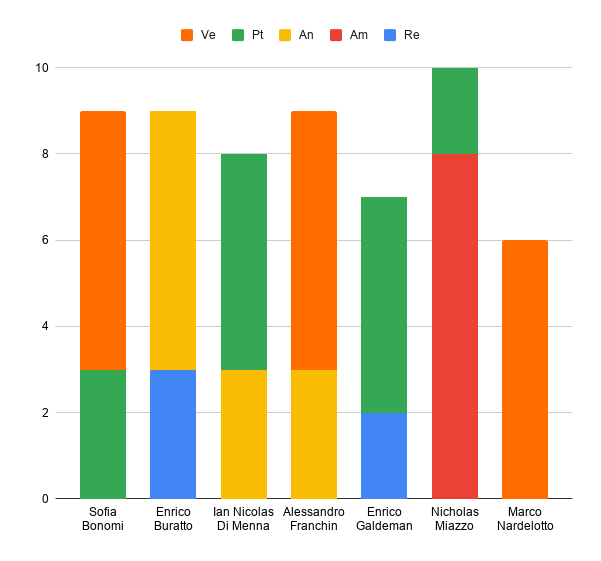
\includegraphics[width=12cm]{img/ore-progettazione.png}
    \caption{Istogramma della distribuzione oraria del periodo di progettazione della technology baseline}
    \label{fig:ore-componente-progettazione}
  \end{figure}

  \subsubsection{Prospetto economico}
  In questo periodo, la suddivisione oraria e i costi per ruolo è la seguente:

  \begin{table}[H]
    \centering
    \begin{tabular}{lcc}
      \rowcolor{lightgray}
      \textbf{Ruolo}  & \textbf{Ore previste} & \textbf{Costo}      \\
Responsabile    & 5                     & € 150,00            \\
Amministratore  & 8                     & € 160,00            \\
Analista        & 12                    & € 300,00            \\
Progettista     & 15                    & € 330,00            \\
Programmatore   & 0                     & € 0,00              \\
Verificatore    & 18                    & € 270,00            \\
\textbf{Totale} & \textbf{58}           & \textbf{€ 1.210,00}
    \end{tabular}
    \caption{Prospetto economico del periodo di progettazione della technology baseline}
  \end{table}


  Per facilitare la lettura della suddivisione oraria per ruolo, i dati vengono rappresentati graficamente mediante il seguente areogramma:
  \begin{figure}[H]
    \centering
    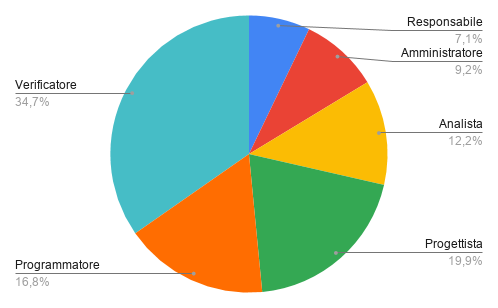
\includegraphics[width=12cm]{img/ruoli-progettazione.png}
    \caption{Areogramma della suddivisione dei ruoli del periodo di progettazione della technology baseline}
    \label{fig:ore-ruolo-progettazione}
  \end{figure}



\end{document}
